% Isabel: alterei o parágrafo abaixo, o original está em comentário, mas não sei se tudo que eu escrevi está correto. É que da maneira como estava escrito tinha duas coisas me “incomodando”: 1) “provided features like”, acho que temos que ser mais “firmes”, não são “características como”, são “as características x, y e z”. 2) “The general opinion from the public about the three selected movies” se não puder ser aplicado para outros filmes, não vejo contribuição no trabalho. Por isso, tentei escrever de forma que ficassem definidas as características, e de forma que mostre que as ferramentas podem ser aplicadas em outros filmes. Também é importante colocar uma referência para "TF-IDF".

%obtained through TF-IDF use. Thus, our focus is to provide the general public opinion about a movie through the mining of some social media. The following subsections contain the description of the used dataset, tools and the developed features.

% Isabel: acho que a descrição do dataset coletado deve estar na próxima seção (eu fiz isso, coloquei na próxima seção). Aqui deve ter a descrição das ferramentas para fazer a coleta. E elas devem estar disponíveis em um github para que outros possam usar também. Acho que "vende melhor" o artigo se mostrarmos que o que fizemos pode ser usado em qualquer outro contexto. Mesmo que os exemplos sejam destes filmes. Portanto, é importante separar o que é a abordagem, da análise feita para o contexto dos filmes desenvolvidos. Comecei esta alteração, vejam o que acham.


For %the context of movie reviews, we decided to 
this work we use data from Twitter and %from the comments on the
YouTube comments. Twitter is used to quickly express opinions, and YouTube is a social media widely used to display trailers. %We developed and used 
Python scripts were developed to gather the desired data from the officials APIs of these social media. 

Comments on Twitter usually use hashtags to indicate their subject. For this reason, we chose to collect data through the use of hashtags instead of using the studio's official page. We believe that, the use of hashtags, would provide a higher number of information and better quality data. The Twitter API implements features that allows the user to provide a hashtag list with the subjects to be collected. Thus for each movie, we selected a different set of hashtags to be collected. From Twitter, we collected: % data like:
%SO: aqui abaixo acho que pode ser uma lista (items) coma  descrição e entre parenteses o nome do variável...
username, lang, screen\_name, text,created\_at, userid,timezone, retweet\_count, id, favorite\_count
The data collected was stored on several JSON files.

%The 
YouTube comments were collected from the Studios' officials channels. We collected data from all the officials' trailers released for a movie. In this analysis, we did not collect data from teasers. We only collected data from the top level of comments on YouTube. We made this decision because, on the other levels the comments, generally, serve as an answer to previous comments and are not properly related to the movie. Our YouTube script only requires the video ID to be executed.

From YouTube script, we collected the following data: 
%SO: mesma coisa que acima... tirar esses "ar de implementação" e deixar com itens descritos e entre parenteses as variaveis.
publishedAt, textOriginal, likeCount, and authorDisplayName'. As the Twitter script, the data is, also, stored in a JSON file.
Both of ours scripts for data collection, along with a detailed description of how to use them, can be found on COLOCAR LINK GITHUB. 
%SO: acima, se é blind não pode colocar link... (nem nomes :)

% Isabel: aqui precisa descrever as ferramentas usadas, os parâmetros que devemos passar (por exemplo, para coletar tweets é preciso colocar as palavras chaves; para o youtube imagino que seja necessário colocar o site) e o resultados gerados (gera um JSON?). Lembrem que quem for ler o artigo tem que conseguir reproduzir o que foi feito. Joana, tem que ver se é blid review ou não. Se não for, tens que ver com o Pedro endereço do github (de preferência ele deve deixar no git do DaVint) do script de coleta do Twitter (talvez seja o caso de referênciar o artigo do DGO). Aproveita e coloca o script de coleta do YouTube no git do DaVInt também. Se for o caso, depois da entrega do artigo pode subir uma nova versão (melhorada) do script, mas se não for blind review, ele deve estar disponível agora. Escrevam um parágrafo para descrever como deve ser feita no Twitter e um sobre a coleta de comentários no YouTube.

IMDB

\subsection{Unsupervised Lexicon-Based Sentiment Analysis}

%JS Ajustes AINDA

% Isabel: abaixo aparece "Sentimental analysis" e "Sentiment Analysis". Acho que seria bom usar sempre a mesma expressão. Abaixo acho que poderiam ter algumas referências no final da frase "Several approaches have already been developed to identify sentiments in texts".
%JS Concordo com a Isabel
Sentiment analysis, also known as opinion mining, is a sub-field of Natural Language Processing (NLP). 
%SO: aqui seria legal uma ref tb
The main purpose of Sentiment Analysis is to identify and extract impressions/opinions from a particular text~\cite{vader}. Several approaches have already been developed to identify sentiments in texts. Some depend on previous annotated data, others rely on polarity lexicons, which is the case for this study. 
%SO: porque ???
%and so we needed to develop mechanisms to overcome this difficulty. To overwhelm the annotated data problem, we resorted to unsupervised learning techniques. Those techniques use ontologies, databases, and lexicons with detailed information about the specific activity.
%SO:acima "tthose techniques"? citar refs...

% In those situations, we need discover another ways to classified this data. Unsupervised Techniques for predicting the sentiment by using ontologies, databases, and lexicons that have detailed information to specific activity are recommend options. 
%Sentimental analysis, also known as opinion mining, is a sub-field of Natural Language Processing (NLP).It's main goal is to identify and extract opinions from a particular text \cite{vader}. There are many approach's to apply sentiment analysis in texts, but when we hadn't labeled training data to learn patterns, that can be a issue. In those situations, we need discover another ways to classified this data. Unsupervised Techniques for predicting the sentiment by using ontologies, databases, and lexicons that have detailed information to specific activity are recommend options. 

% Isabel: colocar referência para paper ou livro que tenha a definiçao de lexicon.
The term polarity lexicon is used to refer to a dictionary or vocabulary with the indications of positive and negative words with an associated score.  Classification techniques are based on word position, surrounding words, context analysis, part-of-speech, phrases, and others. Various lexicons may be used for this analysis.  Examples are: AFINN Lexicon\cite{afinn}, Bing Liu's Lexicon\cite{Jinda}, MPQA subjectivity Lexicon\cite{Wilson}, SentiWordNet\cite{esuli-sentiwordnet}\cite{baccianella-sentiwordnet}, Vader Lexicon\cite{vader}, Pattern Lexicon\cite{pattern}. In the next section we discuss the Vader Lexicon, use in our research. %SO: acima incluir refs please...

% Isabel: particularmente, acho que o vader poderia estar nesta seção, não precisaria ser uma seção separada. Acho que a seção III no momento está com muitas subseções.

%As mentioned, a lexicon is a dictionary or vocabulary, that have a list of positive and negative polar words with some score associate, and using some techniques like the position of words, surrounding words, context, part-of-speech, phrases and etc \cite{Dipanjan:2016}. Various lexicons are used for this analysis, including: AFINN Lexicon, Bing Liu's Lexicon, MPQA subjectivity Lexicon, SentiWordNet, Vader Lexicon, Pattern Lexicon. In the next section will be discuss the Vader Lexicon, chosen for that research. 

% Isabel: a figura abaixo não está sendo referenciada no texto...
\begin{figure*}[t!]
    \begin{center}
    \subfloat[Avengers Infinite War]{{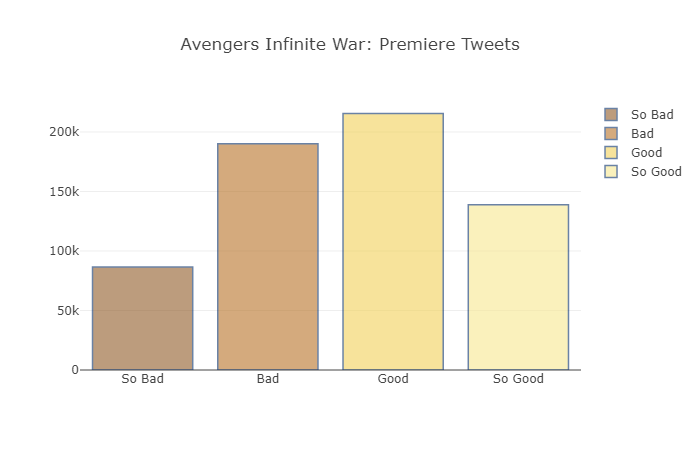
\includegraphics[width=5cm]{img/avengers.png} }}%
    \qquad
    \subfloat[Aquaman]{{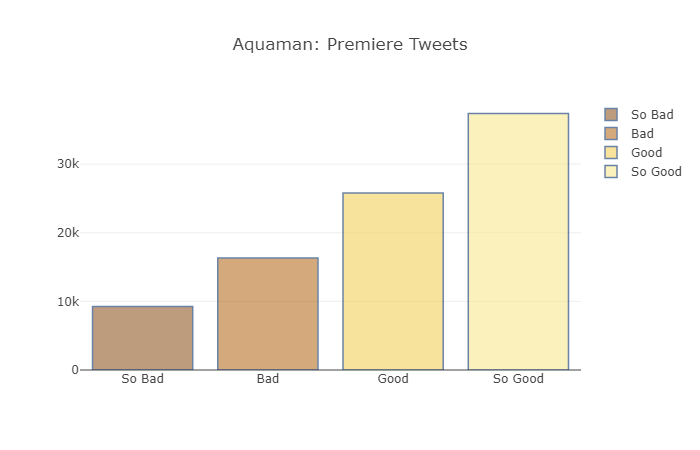
\includegraphics[width=5cm]{img/aquaman.png} }}%
    \qquad
    \subfloat[Captain Marvel]{{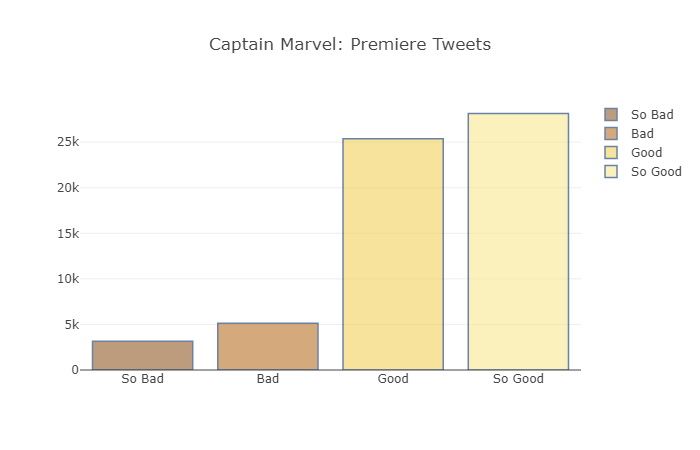
\includegraphics[width=5cm]{img/captain.png} }}%
    \caption{Sentiment Analysis results on the tweets of each movie.}%
    \label{fig:example}%
    \end{center}
\end{figure*}

\subsection{Vader\label{vader}}
%SO: esta subsection não seria dentro da B?
%Ver vitor text ou words
Vader (Valence Aware Dictionary and sEntiment Reasoner) 
%SO: incluir ref
Lexicon is a lexicon based on sentiment-related words. In this approach, each word is labeled according to their semantic orientation as either positive or negative. Vader produces 4 sentiments metrics: the first three (positive, negative and neutral) represent the proportion of the words that match the categories. The final metric, \textit{compound} score, is a combination of the first three metrics normalized.
%SO normalizadas como?
The compound score ranges between -1 and 1, where -1 represents highly negative opinion and 1 highly positive opinion.

%Vader (Valence Aware Dictionary and sEntiment Reasoner) Lexicon is based on lexicon of sentiment-related words. In this approach, each words in the context are generally labeled according to their semantic orientation as either positive or negative. Vader produces 4 sentiments metrics: the first three, positive, negative and neutral, represent the proportion of the texts that matching into ant categories. The final metric, \textit{compound} score, is the sum of first three normalized metrics, between -1 and 1, that -1 represents highly negative and 1 highly positive.

%JS review
Since Vader deals with certain features that most of  other lexicon do not (such as Abbreviations, Upper Case, Emojis, and Special characters), it is considered a very appropriate lexicon to be used in Social Media texts evaluation. 
%SO: ref aqui... consderado por quem?
In the following example, we demonstrate the advantages of using Vader lexicon in Social Media.

%We consider using Vader Lexicon, to evaluate the tweets texts, for supporting the following aspects that non-normalized text may contain: Abbreviations, Upper Case, Emojis, Special characters. To understand, how Vader is great alternative to text analysis, follow a example: 

\begin{figure}[htb]
    \begin{center}
        
\includegraphics[width=0.8\linewidth]{img/Twitter1.png}
    \end{center}
       \caption{Example of a tweet post} %using Vader Lexicon.}
    \label{fig:tweet1}
\end{figure}

The \textit{tweet} presented in Figure~\ref{fig:tweet1} was evaluated with the following scores for sentiment analysis: \textit{'compound'}: 0.6133, \textit{'neg'}: 0.169, \textit{'neu'}: 0.508, \textit{'pos'}: 0.322. As we can see, the overall evaluation of the text denotes a positive emotion. But if this same text was parsed without considering \textit{emojis} and the emotional indication represented by capital letters, 
%SO: mudei um pouco a frase acima para explicar o "capital letters".. mas na verdade não entendi esse parágrafo, fiquei com muitas duvidas. Joana, podes passar aqui?
the scores evaluation would be: \textit{'compound'}: 0.2043, \textit{'neg'}: 0.202, \textit{'neu'}: 0.546, \textit{'pos'}: 0.251. In this case, we can notice a significant drop on the \textit{compound} value, which makes the text's emotion tending to neutral, instead of positive.% as it should.
%SO: tens que explicar o que são esses parametros? compound indica o que?

%The \textit{tweet} shown on Figure \ref{fig:tweet1} presented the following values for the sentiment analysis, \textit{'compound'}: 0.6133, \textit{'neg'}: 0.169, \textit{'neu'}: 0.508, \textit{'pos'}: 0.322, denoting a general positive evaluation (\textit{'compound'}: 0.6133). If the \textit{tweet} was parsed without \textit{emojis} and capital letters were not taken, the values obtained in the evaluation would be: \textit{'compound'}: 0.2043, \textit{'neg'}: 0.202, \textit{'neu'}: 0.546, \textit{'pos'}: 0.251. As we can see, the general evaluation of \textit{tweet} (\textit{compound}) dropped to 0,2043, which, although still a positive value, is closer to the neutral than previously obtained. 


\subsection{TF-IDF\label{TFID}}
%SO: esta sectionj não deveria estar dentro da B tb, como a section c?

\textit{Term Frequency-Inverse Document Frequency} indicates the weight of text's terms according to its frequency proportion~\cite{Dipanjan:2016} across documents. This %technique was developed to be a 
is a well-known metric in information retrieval. %classification metric for searching users' queries results on search engines.

%Term Frequency-Inverse Document Frequency, which indicates the weighting of terms occurring in texts, in proportion your frequency \cite{Dipanjan:2016}. This technique was developed as classification metric, in search results in search engines, based on user queries. 

% Isabel: é preciso explicar que fórmula é essa, para que serve.
%SO: mesmo comentário acima
\begin{equation*}
    W_{t,d} = \left ( \frac{Freq_{t,d}}{Max} \right ) * log_2 \left ( \frac{N}{n_t} \right),
\end{equation*}
where \( W_{t,d}\) represents the term weight \textit{t} in document \textit{d}. 
%SO: não entendi t é termo ou peso (weight?)
\( Freq_{t,d}\) is the number of times that the terms/words ($t$) occur in document \textit{d}. 
%SO: termo e work é a mesma coisa? então seria bom conceituar na primeira vez que aparece
\( Max\) is the term with the highest number of occurrences in the text. 
%SO: Max é o número máximo e não o termo que aparece certo? se sim, corrigir o texto acima...
%JS Rever!!! Vitor
\( N \) is the total of texts in the base of tests, \( n_t \) is the number of texts in the base of tests that owns the term \( t \).

\subsection{Methodology}

% Isabel: alterei o parágrafo abaixo. Original em comentário. Vejam se concordam. Vejam que estou considerando que na seção III-A haverá uma descrição detalhada da coleta. Esta seção III-A  também é referenciada na Seção IV.
%This section 
Figure~\ref{fig:approach} presents our research methodology 
%, which is presented in , and 
which is divided into four steps. The first one consists of collecting data from social media. On this step, we gathered data from both YouTube and Twitter, using the tools described in Subsection~\ref{sec:datasetCollection}. 
%This section will discuss our research approach, described in Figure~\ref{fig:approach}. We divided our research into 4 steps. The first step performed was collecting data from Social Media. On this step, we gathered data from both YouTube and Twitter Social Media, using their officials APIs. From Twitter, we collected the tweets' texts, and from YouTube, we collected the users' comments.
%This section will discuss the research approach proposed, describe in the Figure \ref{fig:approach}. The first step taken is extracting data from social media API's. Text from tweets and youtube's comments are collected, then preprocessing is performed in collection data, including separation of the data in a serie temporal, according to the premiere date, tokenzation and removal links. The stopwords process will not considered in the model, because it acts negatively on the results obtained from Vader Lexicon.

After the data gathering step, we  preprocess the collected data. During this second step, we remove texts' links, distribute the data in a temporal series, and tokenize the text. We do not remove the stopwords because Vader Lexicon uses them on the evaluation process.

On the third step, we use Vader to perform Sentiment Analysis on our texts. This analysis provides us the sentiment scores and compound values (see section \ref{vader}) for the Tweets and comments collected. The texts are then split into several files, according to their polarity. 
%Next, we performed Vader Lexicon to get the Sentiment Score and Compound (mentioned in section \ref{vader}), and after, we realized the data separation in files, according to its polarity. In Data Analysis process, we already have the polarity of each text (sentence), then we calculate TF-IDF in created files, that we know about the important frequency terms in the whole document.
%revisar amanha de manha
The last step of our study is the Data Analysis. On this step, we calculate the TF-IDF (see section \ref{TFID}) statistics using the files generated on the previous step. These statistics provide us information about the most frequent and relevant terms on the documents. We also separate the comments according to its polarity (very positive, positive, negative, and negative).

%On this step, we also 
We generate 3 types of visualization graphics for each one of the Social Medias we chose. The first graphic provides a heatmap, which presents the top XX most commented words for the movie's characters. The second one is a wordcloud, which shows the most used words for each sentiment polarity (very positive, positive, negative and very negative). The third graphic presents a barchart, witch shows the number of comments for each characters. These visualizations can be seen in Figures \cite{} \cite \cite{}
%In Data Analysis process, we already have the polarity of each text (sentence), then we calculate TF-IDF in created files, that we know about the important frequency terms in the whole document.

%To establishing a textual standard, through Pos-Tag (Part-of-Speach) feature, we find for the terms classified as adjectives, within the results from most frequency terms, thus allowing the texts recommendation creation to each movie. 
%SO: lembrar que na introdução dissemos que geramos um meta texto de recomendação. Onde está isto no paper???

\begin{figure*}[htb]
\begin{center}
% \fbox{\rule{0pt}{2in} \rule{.9\linewidth}{0pt}}
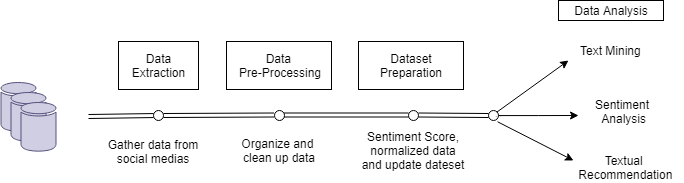
\includegraphics[width=0.8\linewidth]{img/model.png}
\end{center}
   \caption{Proposed approach overview: from data gathering to movie review.}
   % Isabel: a figura é sobre a abordagem, não precisa mencionar os filmes. Por isso alterei a legenda. A original era: Approach overview: Sentiment analysis of the Blockbluster Movies 2018-2019.
\label{fig:approach}
\end{figure*}

% Isabel: lembrar que nas seções abaixo é para descrever o que foi feito, algoritmos e visualizações. Mas, a análise dos filmes deve estar na próxima seção.



